\documentclass[12pt, xcolor=beamer,table,dvipsnames, ignorenonframetext, ngerman]{beamer}
\usetheme{Frankfurt}
\usecolortheme{dove}
\usepackage{appendixnumberbeamer}
%\setbeamersize{text margin left=20pt,text margin right=20pt,}

\beamertemplatenavigationsymbolsempty 
\setbeamertemplate{mini frames}{}
\setbeamertemplate{itemize item}{\textbullet}

\addtobeamertemplate{navigation symbols}{}{
	\ifnum\insertframenumber>\inserttotalframenumber%
	\relax
	\else%
	\usebeamerfont{footline}%
	\usebeamercolor[fg]{footline}%
	\hspace{1em}%
	\insertframenumber
	\fi%
}
\setbeamercolor{footline}{fg=black}
\usepackage{soul}
\makeatletter
\let\HL\hl
\renewcommand\hl{%
	\let\set@color\beamerorig@set@color
	\let\reset@color\beamerorig@reset@color
	\HL}

\usepackage{tipa}
\usepackage{tikz}
\usetikzlibrary{shapes.geometric, arrows}
\mode<presentation>

  \setbeamercovered{invisible}
\usepackage{multicol}
\usepackage[english]{babel}
\usepackage[latin1]{inputenc}
\usepackage{times}
\usepackage[T1]{fontenc}
\usepackage{ulem}
\usepackage{tipa}
\usepackage{qtree}
\usepackage{phonrule}
\usepackage{graphicx}
\usepackage{apacite}
\usepackage{xcolor}
\setlength\parindent{0pt}
\usepackage{natbib}
\usepackage{tikz}
\usetikzlibrary{arrows.meta}
\usepackage{tcolorbox}
\tcbuselibrary{raster}

\title{TODO A-maze works pretty well, actually}
\author{Veronica Boyce}
\date{3 June 2020}

\begin{document}

\begin{frame}
\maketitle
\end{frame}

%Notes for potential Maze presentation:
%
%Goal: introduce A-maze as an option to people, including for people who don't normally do processing; why it might be good
%
%Background:
%- why reaction time
%- existing methods
%- unsatisfied with web results
%
\section{Why RT?}
\begin{frame}{Why measure reading time?}
Linguistic and psycholinguistic theories make predictions about processing difficulty.
\medskip

We assume that harder processing manifests in longer reading/reaction time (RT).
\medskip

RT patterns may be phenomena that theories need to explain.

Examples of harder processing
\begin{itemize}
	\item Less frequent words are harder to retrieve
	\item Reparsing/reanalysis
	\item Less grammatical sentences
\end{itemize}
%certainly not the only measure
%ex. Noisy channel, syntactic preferences, surprisal theory, what's hard in L2.
\end{frame}

\begin{frame}{Two common methods}
%can't get at the internals of processing, so want to use time as proxy for how much is going on 
%but literate humans are good at reading 
\begin{columns}[t]\pause
	\begin{column}{.5\textwidth}
		\begin{center}
			\textbf{\Large Eye-tracking}
			
			\medskip
			
			\includegraphics[width=.9\textwidth]{eye-tracker.jpeg}
			\begin{itemize}
				\item Expensive
				\item Hard to analyse
			\end{itemize}
		\end{center}
	\end{column}\pause
	\begin{column}{.5\textwidth}
		\begin{center}
\textbf{\Large Self-pace reading}

\medskip

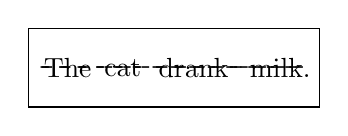
\begin{tikzpicture} %TODO on slide etc
\draw (-.5,-.5) rectangle (3.2,.5);
\onslide<3>{\node at (0,0) {The};}
\onslide<3>{\node at (1.7,0) {- - - - - - - - - - -};}
\onslide<4>{\node at (0,0) {- - - };}
\onslide<4>{\node at (.7,0) {cat};}
\onslide<4>{\node at (2,0) {- - - - - - - - };}
\onslide<5>{\node at (0.3,0) {- - - - - - };}
\onslide<5>{\node at (1.6,0) {drank};}
\onslide<5>{\node at (2.6,0) {- - - -};}
\onslide<6->{\node at (.9,0) {- - - - - - - - - - -};}
\onslide<6->{\node at (2.7,0) {milk.};}
\end{tikzpicture}
\end{center}
			\begin{itemize}
	\item Lots of spillover
	\item Messy data 
\end{itemize}
\end{column}
\end{columns}

\end{frame}

\begin{frame}{Maze Task}
\centering
\tikzset{
	font={\fontsize{14pt}{12}\selectfont}}
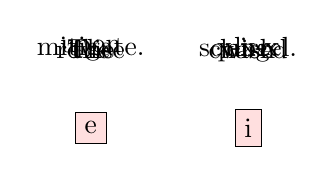
\begin{tikzpicture}
\onslide<1->{\node[draw] (a) at (-1,-.5) {e};}
\onslide<1->{\node[draw] (b) at (1,-.5) {i};}
\onslide<1-2>{\node  (c) at (-1,.5) {The};}
\onslide<1-2>{\node  (d) at (1,.5) {x-x-x};}
\onslide<3-4>{\node  (c) at (-1,.5) {upon};}
\onslide<3-4>{\node  (d) at (1,.5) {dog};}
\onslide<5-6>{\node  (c) at (-1,.5) {revise};}
\onslide<5-6>{\node  (d) at (1,.5) {chased};}
\onslide<7-8>{\node  (c) at (-1,.5) {the};}
\onslide<7-8>{\node  (d) at (1,.5) {wish};}
\onslide<9-10>{\node  (c) at (-1,.5) {mitigate.};}
\onslide<9-10>{\node  (d) at (1,.5) {squirrel.};}
\onslide<2,8>{\node[draw, fill=pink!50] at (a) {e};}
\onslide<4,6,10>{\node[draw, fill=pink!50] at (b) {i};}
\end{tikzpicture}
\end{frame}

\begin{frame}{A third option: Maze}
\begin{columns}
	\begin{column}{0.5\textwidth}
		\begin{center}
		\textbf{\large G-maze}
		\includegraphics[clip, trim=9cm 14cm 11cm 1cm,width=.9\textwidth]{gmaze.pdf}
		\end{center}
	
	\end{column}
	\begin{column}{0.5\textwidth} 
		\begin{center}
		\textbf{\large L-maze}
			\includegraphics[clip, trim=9cm 14cm 11cm 1cm,width=.9\textwidth]{lmaze.pdf}
		\end{center}
	\end{column}
\end{columns}

\medskip

Sentence ends when a mistake is made

Central claim: forces extremely incremental processing (no spillover)

\begin{flushright}
	{\small(Forster et al. 2009; Witzel et al. 2012)}
\end{flushright}
\end{frame}

\section{Experiment 1a}
\begin{frame}{Web Maze}
Maze well suited to run on the web.
\begin{itemize}
	\item Implement in Ibex using js
\end{itemize} 

Test by replicating Witzel et al. (2012)
\begin{itemize}
	\item Comparison of eye-tracking, SPR, L-maze, G-maze (all in-lab)
	\item Got materials and data from original
	\item Run SPR, L-maze, and G-maze on MTurk
\end{itemize}
\end{frame}

\begin{frame}{Materials}

\textbf{Relative Clause}

\sethlcolor{green}
\textit{Low:} The son of the \uline{lady} who politely introduced \hl{herself} was popular at the party.
\sethlcolor{pink}

 \textit{High:} The \uline{son} of the lady who politely introduced \hl{himself} was popular at the party.
 

\textbf{Adverb Clause}

\sethlcolor{green}\textit{Low:} James will fix the car he \uline{drove} \hl{yesterday}, but he will need some help.

\sethlcolor{pink} \textit{High:} James \uline{will fix} the car he drove \hl{tomorrow}, but he will need some help.
		
\textbf{Sentence v Noun Phrase conjunction}

\sethlcolor{green} \textit{Comma:} The swimmer disappointed her \uline{coach}, and her mother \hl{tried} to console her.

\sethlcolor{pink}
\textit{No comma:} The swimmer disappointed her \uline{coach} and her mother \hl{tried} to console her.
\end{frame}

\begin{frame}{Results}
\begin{small}	
	\sethlcolor{green}
The son of the lady who politely introduced \hl{herself}\sethlcolor{pink} / \hl{himself} was popular at the party.
	
\end{small}
\includegraphics[width=\textwidth]{g_rel.pdf}
\end{frame}

\begin{frame}{Results}
\begin{small}	

\sethlcolor{green}James will fix the car he drove \hl{yesterday}\sethlcolor{pink} / \hl{tomorrow},  but he will need some help.

\end{small}
\includegraphics[width=\textwidth]{g_adv.pdf}
\end{frame}

\begin{frame}{Results}
\begin{small}	
\sethlcolor{green}The swimmer disappointed her coach\hl{,} and her mother \hl{tried} / \sethlcolor{pink}\hl{tried} to console her.
\end{small}
\includegraphics[width=\textwidth]{g_svnp.pdf}
\end{frame}
\begin{frame}
Good news: G-maze work over the web

Bad news: G-maze materials are a huge pain to write
\end{frame}

\section{A-maze}

\begin{frame}{Meanwhile in NLP}
Language models (LM)
\begin{itemize}
	\item Trained on large corpora to predict the next word
	\item Learn the distribution over next word given a partial sentence
\end{itemize}
Surprisal: negative log probability
\begin{itemize}
	\item 2 bits of surprisal = 1/4
	\item 10 bits of surprisal $\approx$ 1/1000 
	\item +1 surprisal = half as likely
\end{itemize}
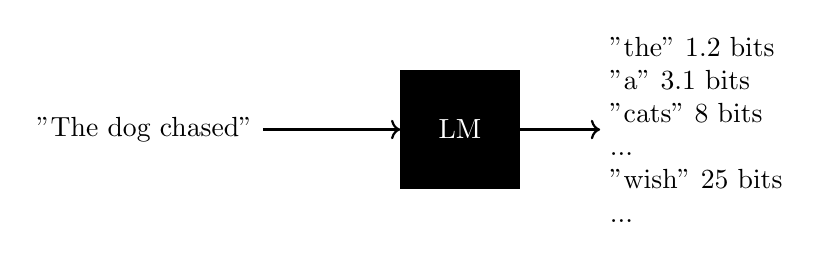
\begin{tikzpicture}
\node (A) at (0,0) {"The dog chased"};
\node  (B) at (4,0) [draw, minimum width=1.5cm, minimum height=1.5cm, fill=black] {\textcolor{white}{LM}} ;
\draw [->, thick] (A) -- (B); 
\node[align=left] (C) at (7,0) {"the" 1.2 bits \\"a" 3.1 bits\\"cats" 8 bits\\...\\"wish" 25 bits\\...};
\draw [->, thick] (B) -- (C); 
\end{tikzpicture}
\end{frame}

\begin{frame}{LMs as RAs}
Feed items to LM, get out distribution and choose a high-surprisal word for the distractor.

Want to avoid random nonsense, so we restrict distractor options
\begin{itemize}
	\item Use a dictionary, do some manual exclusions
	\item Match distractor's length, frequency to correct word
	\item Go down list of potential distractors until we find one that's high enough surprisal
\end{itemize}

\end{frame}

\section{Experiment 1b}
\begin{frame}{But does it work?}
Foreshadowing: Yes.
\end{frame}

\begin{frame}{But does it work?}
Test with 2 pre-trained LSTM models (Gulordava 
Go back to these syntactic things. Add A-maze results. Ran them didn't look at them. 
\end{frame}

\begin{frame}{But does it work?}
\includegraphics[width=.95\textwidth]{a_all.pdf}
\end{frame}
%
%\begin{frame}{Caveats}
%there were a lot of mistakes on word 2
% - can't tell if this is bad participants or bad distractors
% - presumably some of each
% - data loss, want to fix this
% - can't really tell how good participants are,
%\end{frame}
%
%\begin{frame}
%Solution 1:
%make it better
%
%we did a little of this, added some tweaks, made is easier for users to specify badnesses
%
%but this is hard, it's unclear what to expect, and we haven't done grid search or anything
%\end{frame}
%
%\begin{frame}
%Solution 2: `redo mode`
%Just have people correct their mistakes and keep going. 
%\end{frame}
%
%\begin{frame}{Maze with Error Correction}
%\centering
%\tikzset{
%	font={\fontsize{14pt}{12}\selectfont}}
%\begin{tikzpicture}
%\onslide<1->{\node[draw] (a) at (-1,-.5) {e};}
%\onslide<1->{\node[draw] (b) at (1,-.5) {i};}
%\onslide<1-2>{\node  (c) at (-1,.5) {The};}
%\onslide<1-2>{\node  (d) at (1,.5) {x-x-x};}
%\onslide<3-4>{\node  (c) at (-1,.5) {upon};}
%\onslide<3-4>{\node  (d) at (1,.5) {dog};}
%\onslide<5-8>{\node  (c) at (-1,.5) {revise};}
%\onslide<5-8>{\node  (d) at (1,.5) {chased};}
%\onslide<9-10>{\node  (c) at (-1,.5) {the};}
%\onslide<9-10>{\node  (d) at (1,.5) {wish};}
%\onslide<11-12>{\node  (c) at (-1,.5) {mitigate.};}
%\onslide<11-12>{\node  (d) at (1,.5) {squirrel.};}
%\onslide<2,6,10>{\node[draw, fill=pink!50] at (a) {e};}
%\onslide<4,8,12>{\node[draw, fill=pink!50] at (b) {i};}
%\onslide<7,8>{\node[text=red] at (0,-1.5) {\small Incorrect. Please try again.};}
%\end{tikzpicture}
%\end{frame}
%
%\begin{frame}
%\includegraphics{maze_diagram.pdf} %TODO trim
%- really easy to do in our framework
%and now we have a lot of advantages
%- have all the data
%so we can tell the bad participant from the bad item
%and the bad distractor doesn't screw us over
%
%Convenient side effect: we can run multi-sentence items. Hadn't been done before b/c even low error rates add up.
%\end{frame}
%
%\section{Experiment 2}
%
%\begin{frame}{Natural Stories}
%Natural stories corpus
%10 stories, each about 1000 words
%read fluently to native speakers
%sample,
%and they come with comprehension questions
%\end{frame}
%
%\begin{frame}{Natural Stories}
%Methods
%- read a short practice w comp q
%- read 1 story and questions
%\end{frame}
%
%\begin{frame}{Natural Stories}
%Methods
%- read a short practice w comp q
%- read 1 story and questions
%\end{frame}
%
%\begin{frame}{Natural Stories}
%Participant quality
%- mean RT versus how many they got right
%- select this part and not those
%\includegraphics{error.pdf}
%\end{frame}
%\begin{frame}{Natural Stories}
%Participant quality and comprehension questions
%\includegraphics{comp.pdf}
%\end{frame}
%
%\begin{frame}{Natural Stories}
%It's working
%- people will put up with reading this for 15 minutes
%- some of them can understand the story
%- our distractors are actually good enough (most of the time)
%\end{frame}
%
%\begin{frame}{Natural Stories}
%Analysis time -- we check for known surprisal effects
%length*surprisal (? frequency)
%Copy over table 
%spillover
%is it linear
%what we find
%\includegraphics[]{gam.pdf}	
%note that it's crucial to use single token words -- predictions on add punct together aren't good
%\end{frame}
%
%\begin{frame}{Natural Stories}
%And it same result holds on after-mistake data 
%skip a couple words where people might be recovering (double check how much we skip), but then it's fine
%\end{frame}
%
%\section{Conclusion}
%\begin{frame}
%Potential and Unknowns
%- easily extendable to other language models, languages 
%- easy to use; command line runnable, backed by Python
%
%Unknowns:
%- only as good as the lms are, might not be great for triple center embeddings ... but you can also fix a few words
%\end{frame}

%


\appendix
%Back pocket slide on matching procedure
%back pocket on more on model results??
%do we even need back pockets??

\end{document}

